\subsubsection{16.12.2015}
\textit{\textbf{Time frame:}} 16:00-22:00 \newline
The mechanism for shifting the bucket was recreated with relation to the lastest version. In contrast, in the new version there were applied longer slats (40 cm), that will provide enough offset of the bucket. Also, the mount of the mechanism was made of aluminium profile instead of tetrix parts in order to save weight.

\begin{figure}[H]
	\begin{minipage}[h]{0.58\linewidth}
		\center{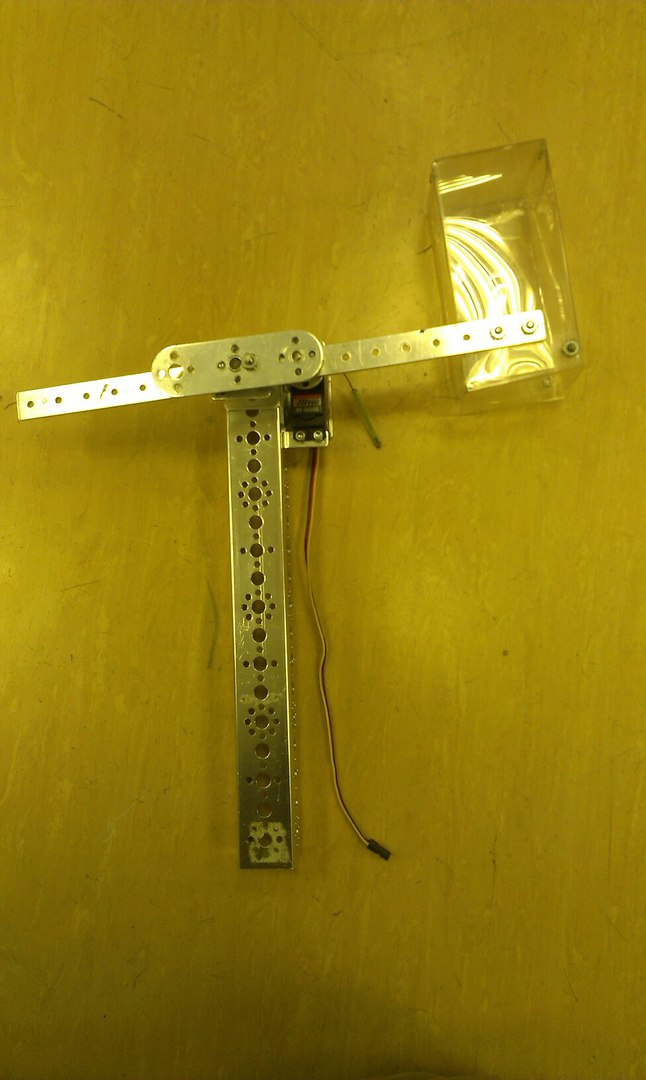
\includegraphics[scale=0.2]{3Engineering/5Team_meetings/days_of_meetings/2015.11.17/images/01}}
		\caption{Winch installed onto the carriage}
	\end{minipage}
	\hfill
	\begin{minipage}[h]{0.37\linewidth}
		\center{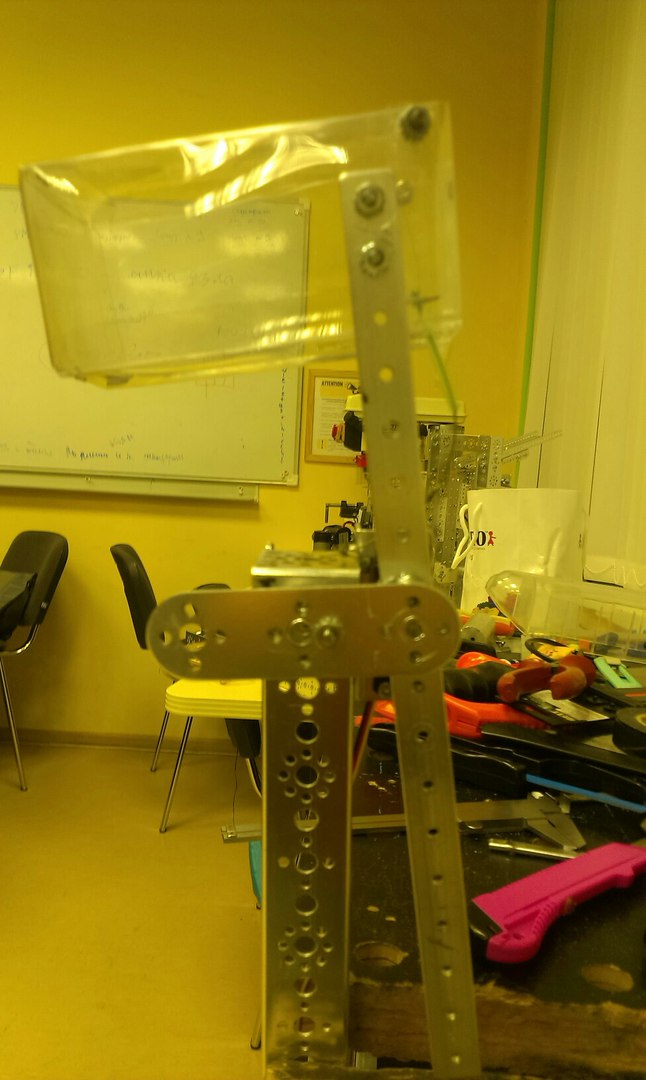
\includegraphics[scale=0.22]{3Engineering/5Team_meetings/days_of_meetings/2015.11.17/images/02}}
		\caption{The construction of the winch}
	\end{minipage}
\end{figure}
